\documentclass{article}
\usepackage[OT4]{fontenc}
\usepackage[polish]{babel}
%\usepackage{polski}
\usepackage[utf8]{inputenc}
\usepackage{apacite}
\usepackage{natbib}
\usepackage{caption}
\usepackage{booktabs}
\usepackage{colortbl, xcolor}
\usepackage{tabularx}
\usepackage{graphicx}
\usepackage{multirow}
\usepackage{epstopdf}

\author{Michał Burdukiewicz, Przemysław Gagat}
\title{Tworzenie skróconych alfabetów aminokwasowych dla białek 
amyloidogennych\linebreak \vskip{} 
\large{Projekt badawczy Doktoranckiego Koła Naukowego Bioinformatyki}} 
\date{}

\AtBeginDocument{%
  \renewcommand{\tablename}{Tab.}
} 

\AtBeginDocument{%
  \renewcommand{\figurename}{Tab.}
} 

\begin{document}

\maketitle

\section{Założenia projektu badawczego}

Sekwencje białkowe zazwyczaj są opisywane przy wykorzystaniu alfabetu 
aminokwasowego zawierającego 20 aminokwasów. W przypadku wielu problemów 
badawczych, np. przewidywania funkcji białka~\citep{longo_simplified_2013} lub 
jego fałdowania~\citep{murphy_simplified_2000}, znajomość dokładnego składu 
aminokwasowego nie jest konieczna i trafnych analiz można dokonywać na podstawie 
skróconego alfabetu aminokwasego.

Skrócony alfabet aminokwasowy to alfabet w którym aminokwasy na podstawie 
określonych podobieństw są przypisane do grup (Tab.~\ref{tab:przykladowy}). 
W sekwencji białkowej zapisanej przy użyciu takiego alfabetu konkretne reszty 
aminokwasowe zastępuje się numerem grupy do której zostały przypisane.
Zazwyczaj w celu stworzenia skróconego alfabetu wykorzystuje się macierze 
podstawień~\citep{cannata_simplifying_2002} lub właściwości fizykochemiczne 
aminokwasów~\citep{stephenson_unearthing_2013}. Istnieją również
kryteria pozwalające ustalić optymalną wielkość alfabetu (liczbę grup, do 
których przypisujmy aminokwasy)~\citep{solis_amino_2015}.

% latex table generated in R 3.3.1 by xtable 1.8-2 package
% Thu Jul 14 09:41:13 2016
\begin{table}[ht]
\centering
\caption{Przykładowy skrócony alfabet 
aminokwasowy~\citep{melo_accuracy_2006}. Sekwencja ADPH w tym alfabecie 
zostanie zapisana jako 1335.} 
\begin{tabular}{rl}
  \toprule
Numer grupy & Aminokwasy \\ 
  \midrule
  1 & A, G \\ 
   \rowcolor[gray]{0.85}  2 & C \\ 
    3 & D, E, K, N, P, Q, R, S, T \\ 
   \rowcolor[gray]{0.85}  4 & F, I, L, M, V, W, Y \\ 
    5 & H \\ 
   \bottomrule
\end{tabular}
\label{tab:przykladowy}
\end{table}

Nasze wstępne wyniki sugerują, że w przypadku niektórych problemów 
przewidywania właściwości białek, zastosowanie skróconego alfabetu 
aminokwasowego może znacząco ulepszyć precyzję predykcji. Jednakże taki alfabet  
musi zostać wybrany spośród wielu potencjalnych skróconych alfabetów. Liczba 
wszystkich możliwych skróconych alfabetów aminokwasowych $n_s$ zawierających $k$ 
grup jest wyrażona poprzez: 

$$ n_s = \frac{1}{k!} \sum^{k}_{j = 0} (-1)^{k-j}  {k \choose j} j^{20} $$

Nawet przy założeniu, że optymalna wielkość skróconego alfabetu jest już znana, 
to liczba potencjalnych możliwości jest bardzo duża (np. wszystkich alfabetów 
sześcioelementowych jest $4.306079 \times 10^{12}$).

\section{Obecny stan badań}

\subsection{Predykcja białek amyloidogennych}

Jednym z poprzednich zadań badawczych naszego Koła było opracowanie algorytmu 
przewidującego amyloidy, białka, których agregaty występują w różnych 
zaburzeniach neurodegeneracyjnych (m.in. choroby Alzheimera, 
Creutzfelda-Jacoba). Podczas tworzenia predyktora amyloidogenności AmyloGram 
wygenerowaliśmy i przetestowaliśmy 18 535 unikalnych skróconych alfabetów o 
długości od 3 do 6 (ok. $3.63 \times 10^{-7} \% $ wszystkich możliwych 
skróconych alfabetów o długości od 3 do 6). Spośród sprawdzonych alfabetów 
wybrano ten, który gwarantował najlepszą predykcję. 

Zastosowanie skróconego alfabetu istotnie podwyższyło skuteczność przewidywania 
amyloidogenności (Tab. \ref{tab:alfabety}). Jednakże ze względu na szczupłość 
sprawdzonego zbioru alfabetów, prawdopobnie istnieje skrócony alfabet, który 
pozwala na jeszcze lepsze predykcje oraz precyzyjniejsze opisanie procesu 
agregacji białek amyloidowych.

\begin{table}[ht]
\centering
\small
\caption{Porównanie predykcji amyloidogenności na zbiorze testowym 
\textit{pep424}~\citep{walsh_pasta_2014} dla klasyfikatorów uczonych na 
sekwencjach zapisanych z wykorzystaniem pełnego alfabetu i skróconego. AUC: Area 
Under the Curve. MCC: Matthew's Correlation Coefficient.} 
\label{tab:alfabety}
\begin{tabular}{ccccc}
  \toprule
Classifier & AUC & MCC  \\ 
  \midrule
Skrócony alfabet (zbiór uczący A) & 0.8856 & 0.6057  \\
   \rowcolor[gray]{0.85}Pełny alfabet (zbiór uczący A) & 0.8411 & 0.5427 \\ 

Skrócony alfabet (zbiór uczący B) & \textbf{0.8972} & \textbf{0.6307}  \\ 
  \rowcolor[gray]{0.85}Pełny alfabet (zbiór uczący B) & 0.8581 & 0.5698 
\\ 
Skrócony alfabet (zbiór uczący C) & 0.8728 & 0.5420 
\\
   \rowcolor[gray]{0.85}Pełny alfabet (zbiór uczący C) & 0.8610 & 0.5490 & \\
   \bottomrule
\end{tabular}
\end{table}

\subsection{Predykcja peptydów sygnałowych u nietypowych organizmów}

Zredukowane alfabety aminokwasowe zostały również wykorzystane w 
naszym programie signalHsmm, który przewiduje występowanie peptydów sygnałowych 
u Eukariontów. Zastosowanie skróconego alfabetu aminokwasowego pozwoliło 
trafnie przewidywać peptydy sygnałowe również u nietypowych grup taksonomicznych 
takich jak rodzaj \textit{Plasmodiidae} do którego zalicza się zarodziec 
malarii. Nietypowy skład aminokwasowy takich peptydów sygnałowych utrudnia ich 
rozpoznawanie przy użyciu innych programów, które wykorzystują pełny alfabet 
aminokwasowy. Zapisanie sekwencji peptydów sygnałowych \textit{Plasmodiidae} 
przy użyciu skróconego alfabetu aminokwasowego pozwala na identyfikację reguł 
decyzyjnych, które łączą je z analogicznymi sekwencjami pochodzącymi od innych 
eukariontów (Rys.~\ref{fig:PCA}). Nie jest to możliwe przy użyciu pełnego 
alfabetu aminokwasowego.

\begin{figure}[htbp]
\centering
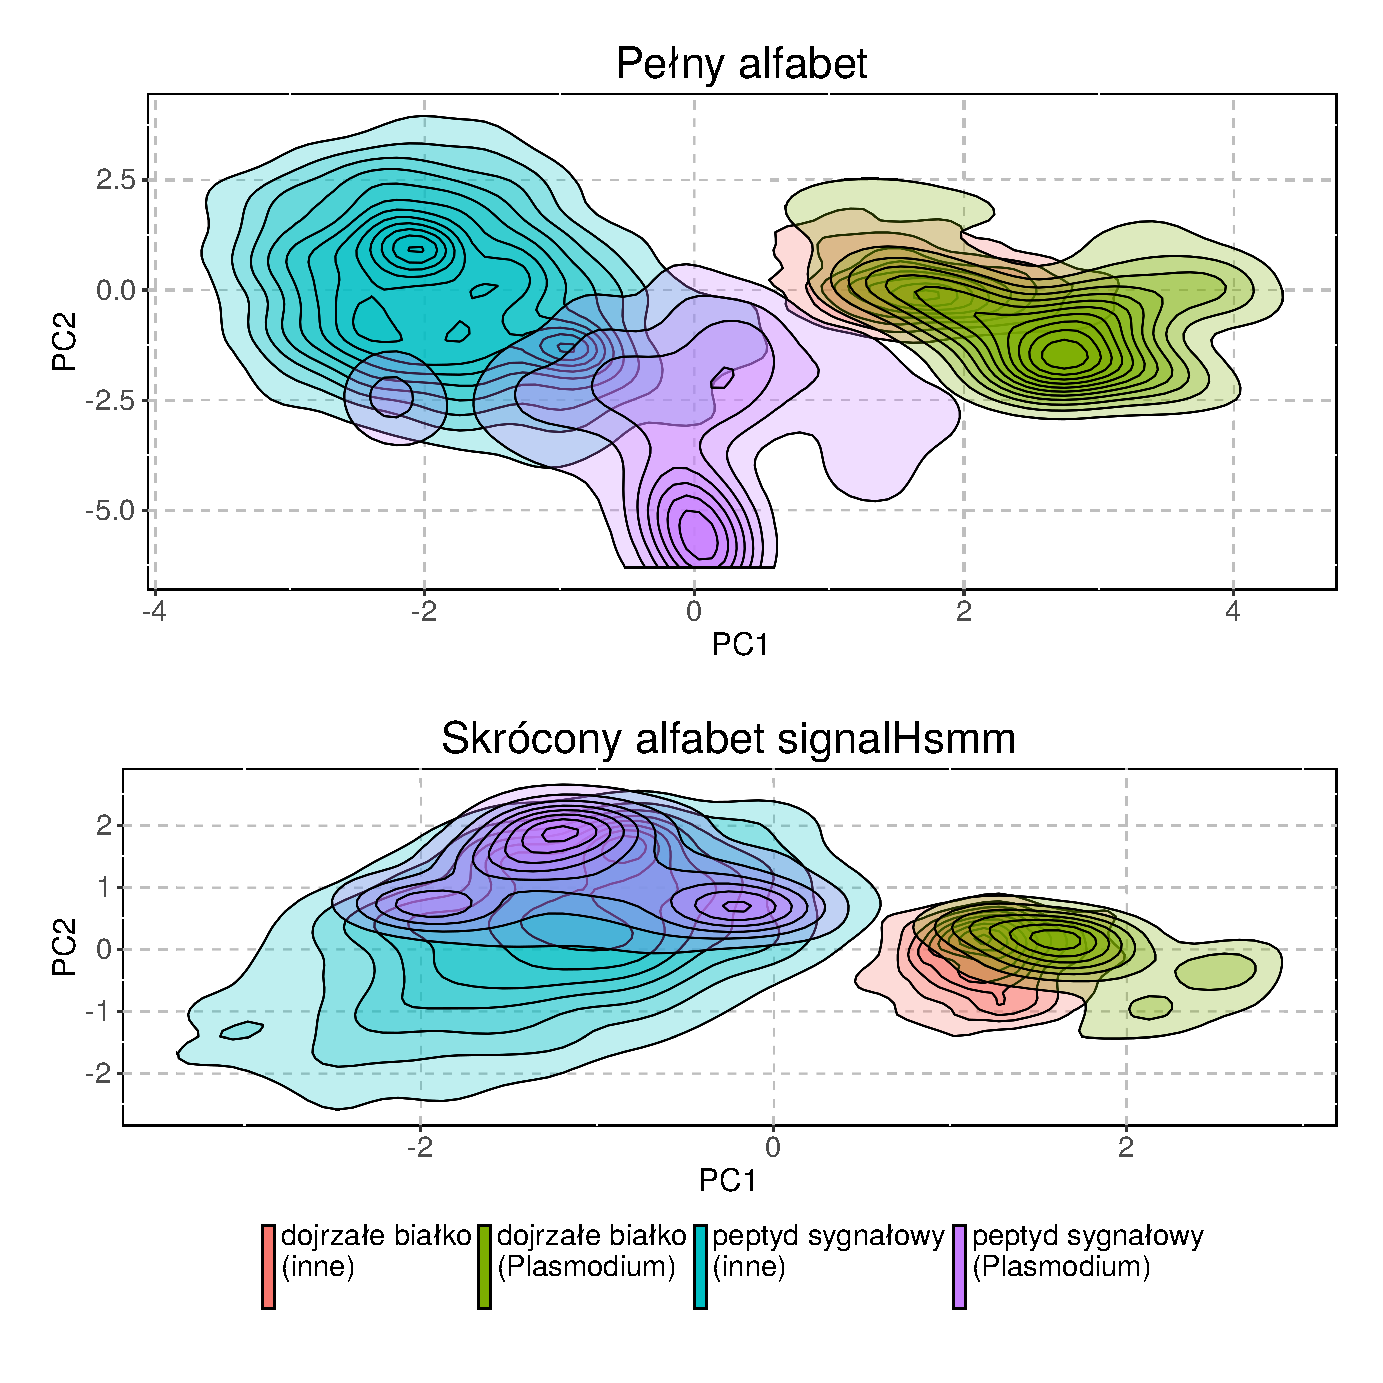
\includegraphics[width=0.7\textwidth]{signalHsmm.eps}
\caption{Wyniki PCA dla częstości aminokwasów w peptydach sygnałowych i 
dojrzałych białkach \textit{Plasmodiidae} oraz innych eukariontów.}
\label{fig:PCA}
\end{figure}


\section{Cel badań}

Głównym zadaniem badawczym jest opracowanie nowej metody poszukiwania 
skróconych alfabetów amyloidogennych. Nowe rozwiązania zostaną zastosowane do 
problemu przewidywania białek amyloidogennych i nietypowych peptydów 
sygnałowych.

\section{Metody}

Głównym narzędziem wykorzystywanym w projekcie badawczym jest pakiet 
\textit{biogram} przeznaczony do analizy n-gramowej sekwencji biologicznych. 
Program ten zawiera liczne narzędzia umożliwiające tworzenie i porównywanie 
skróconych alfabetów (takie jak \textit{similarity 
index})~\citep{stephenson_unearthing_2013}, które mogą być podstawą dla nowego 
algorytmu opracowanego podczas projektu badawczego.


\section{Planowane wydatki}

Łączny koszt projektu badawczego to 29 802,00 zł.

\begin{table}[!htbp]
\centering
\caption*{Kosztorys projektu badawczego.}
\begin{tabular}{rrr}
\cline{1-2}
\multicolumn{1}{|c}{Nazwa}                                   & \multicolumn{1}{|c|}{Koszt}   &  \\ \cline{1-2}
\multicolumn{1}{|c}{Utworzenie studenckiego klastra obliczeniowego} & 
\multicolumn{1}{|c|}{25 042,00 zł} &  \\ \cline{1-2}
\multicolumn{1}{|c}{Akcesoria niezbędne w realizacji zadań badawczych}   & 
\multicolumn{1}{|c|}{760,00 zł} &  \\ \cline{1-2}
\multicolumn{1}{|c}{Wyjazdy konferencyjne}   & 
\multicolumn{1}{|c|}{4 000,00 zł} &  \\ \cline{1-2}
Łącznie    & 29 802,00 zł                    & 
\end{tabular}
\end{table}

\subsection{Utworzenie studenckiego klastra obliczeniowego}

Realizacja projektu wymaga stworzenia nowego klastra obliczeniowego na potrzeby 
przewidzianych zadań badawczych (Tab.~\ref{tab:klaster}). Po zakończeniu badań 
klaster pozostanie cennym narzędziem dla studentów, którzy będą go mogli 
wykorzystać do obliczeń niezbędnych do napisania prac dyplomowych.

\begin{table}[]
\centering
\caption{Koszty utworzenia studenckiego klastra obliczeniowego.}
\label{tab:klaster}
\begin{tabular}{ccccl}
\cline{1-4}
\multicolumn{1}{|c|}{Nazwa}                                                      
                          & \multicolumn{1}{c|}{Cena (szt.)} & 
\multicolumn{1}{c|}{Liczba} & \multicolumn{1}{c|}{Łączna cena}  & 
\multicolumn{1}{c}{} \\ \cline{1-4}
\multicolumn{1}{|c|}{Zasilacze - 500W}                                           
                          & \multicolumn{1}{c|}{230,00 zł}   & 
\multicolumn{1}{c|}{4}      & \multicolumn{1}{c|}{920,00 zł}    & 
\multicolumn{1}{c}{} \\ \cline{1-4}
\multicolumn{1}{|c|}{Bateria do UPS APC RBC7}                                    
                          & \multicolumn{1}{c|}{314,00 zł}   & 
\multicolumn{1}{c|}{3}      & \multicolumn{1}{c|}{942,00 zł}    & 
\multicolumn{1}{c}{} \\ \cline{1-4}
\multicolumn{1}{|c|}{\begin{tabular}[c]{@{}c@{}}Napęd optyczny \\ zewnętrzny USB 
2.0\end{tabular}}         & \multicolumn{1}{c|}{150,00 zł}   & 
\multicolumn{1}{c|}{1}      & \multicolumn{1}{c|}{150,00 zł}    &                
      \\ \cline{1-4}
\multicolumn{1}{|c|}{\begin{tabular}[c]{@{}c@{}}Switch Netgear GS324 \\ 24 porty 
10/100/1000\end{tabular}} & \multicolumn{1}{c|}{500,00 zł}   & 
\multicolumn{1}{c|}{2}      & \multicolumn{1}{c|}{1 000,00 zł}  &                
      \\ \cline{1-4}
\multicolumn{1}{|c|}{Pamięć RAM 2x8GB DDR3}                                      
                          & \multicolumn{1}{c|}{330,00 zł}   & 
\multicolumn{1}{c|}{1}      & \multicolumn{1}{c|}{330,00 zł}    &                
      \\ \cline{1-4}
\multicolumn{1}{|c|}{Jednostka obliczeniowa (komputer)}                          
                          & \multicolumn{1}{c|}{3 500,00 zł} & 
\multicolumn{1}{c|}{6}      & \multicolumn{1}{c|}{21 000,00 zł} &                
      \\ \cline{1-4}
\multicolumn{1}{|c|}{Monitor 24''}                                               
                          & \multicolumn{1}{c|}{700,00 zł}   & 
\multicolumn{1}{c|}{1}      & \multicolumn{1}{c|}{700,00 zł}    &                
      \\ \cline{1-4}
                                                                                 
                          &                                  & Łącznie:          
          & 25 042,00 zł                       & \multicolumn{1}{c}{}
\end{tabular}
\end{table}

\subsection{Akcesoria niezbędne w realizacji zadań badawczych}

Właściwe zrealizowanie projektu badawczego wymaga również dokupienie 
akcesoriów (Tab.~\ref{tab:akcesoria}), takich jak pamięci USB niezbędne do 
przenoszenia duzych objętości danych i słuchawki z mikrofonem do prowadzenia 
rozmów z zagranicznym uczestnikiem projektu. Wykonanie części zadań badawczych 
nie byłaby możliwa gdyby nie komputery przenośne udostępnione członkom Koła 
przez Zakład Genomiki. Bezpieczny transport otrzymanego sprzętu wymaga zakupu 
specjalnych plecaków na laptopy.

\begin{table}[]
\centering
\caption{Koszty akcesoriów niezbędnych w realizacji zadań badawczych.}
\label{tab:akcesoria}
\begin{tabular}{ccccc}
\cline{1-4}
\multicolumn{1}{|c|}{Nazwa}                           & \multicolumn{1}{c|}{Cena 
(szt.)} & \multicolumn{1}{c|}{Liczba} & \multicolumn{1}{c|}{Łączna cena} &       
               \\ \cline{1-4}
\multicolumn{1}{|c|}{Pendrive USB 3.0 - 32 GB}        & 
\multicolumn{1}{c|}{45,00 zł}    & \multicolumn{1}{c|}{4}      & 
\multicolumn{1}{c|}{180,00 zł}   &                      \\ \cline{1-4}
\multicolumn{1}{|c|}{Słuchawki z mikrofonem Creative} & 
\multicolumn{1}{c|}{140,00 zł}   & \multicolumn{1}{c|}{2}      & 
\multicolumn{1}{c|}{280,00 zł}   &                      \\ \cline{1-4}
\multicolumn{1}{|c|}{Plecak na laptopa}               & 
\multicolumn{1}{c|}{150,00 zł}   & \multicolumn{1}{c|}{2}      & 
\multicolumn{1}{c|}{300,00 zł}   & \multicolumn{1}{l}{} \\ \cline{1-4}
                                                      &                          
        & Łącznie:                    & 760,00 zł                        &       
              
\end{tabular}
\end{table}

\subsection{Wyjazdy konferencyjne}

Wstępne wyniki badań zostaną zaprezentowane podczas 9 Sympozjum Polskiego 
Towarzystwa Bioinformatycznego (28-30 września 2016, Białystok) oraz European R 
User Meeting (12-14 października 2016, Poznań). Dofinansowanie 
umożliwi większej liczbie członków Koła aktywny udział w konferencji i 
zaprezentowanie nie tylko wyników realizacji zadań badawczych postawionych w tym 
wniosku, ale również postępów w realizacji prac doktorskich. W ramach projektu 
łącznie odbędą się cztery wyjazdy (trzy wyjazdy na Sympozjum Polskiego 
Towarzystwa Bioinformatycznego i jeden wyjazd na European R 
User Meeting).

\begin{table}[!htbp]
\centering
\caption*{Kosztorys wyjazdów zagranicznych.}
\begin{tabular}{lllll}
\cline{1-4}
\multicolumn{1}{|c|}{Nazwa}                     & \multicolumn{1}{c|}{Cena (szt.)} & \multicolumn{1}{c|}{Liczba} & \multicolumn{1}{c|}{Łączna cena} &  \\ \cline{1-4}
\multicolumn{1}{|c|}{Dofinansowanie wyjazdu} & \multicolumn{1}{c|}{1 000 zł}    
 & \multicolumn{1}{c|}{4}      & \multicolumn{1}{c|}{4 000 zł}     &  \\ 
\cline{1-4}
                                                &                                
  & Łącznie:                    & 4 000,00 zł                          & 
\end{tabular}
\end{table}


\bibliographystyle{apacite} 
\bibliography{biogram_pub}

\end{document}